\section{Gathering of Data}

I used the  \href{https://www.kaggle.com/Cornell-University/arxiv}{Arxiv} and Neural Information Processing 
    Systems (\href{https://www.kaggle.com/benhamner/nips-papers}{NIPS}) datasets from kaggle. On listing \ref{schemas}
we can see raw schema of the files. Arxiv in json format and NIPS is on csv files. I hosted both files on a S3: 
\emph{s3a://arxivs3/input\_data/arxiv-metadata-oai-snapshot.json}, \emph{s3a://arxivs3/input\_data/NIPS.csv}. To upload the
data to s3, I had to create an EC2 instance, install \emph{miniconda}, \emph{kaggle} library and aws client (see listing \ref{transfer}). 
   
\begin{mdframed}[backgroundcolor=light-gray, roundcorner=10pt,leftmargin=1, rightmargin=1, innerleftmargin=15, innertopmargin=15,innerbottommargin=15, outerlinewidth=1, linecolor=light-gray]
\begin{lstlisting}[caption={Datasets Schema},label={schemas}]    
>>> df_arxiv.printSchema()
root
 |-- abstract: string (nullable = true)
 |-- authors: string (nullable = true)
 |-- authors_parsed: array (nullable = true)
 |    |-- element: array (containsNull = true)
 |    |    |-- element: string (containsNull = true)
 |-- categories: string (nullable = true)
 |-- comments: string (nullable = true)
 |-- doi: string (nullable = true)
 |-- id: string (nullable = true)
 |-- journal-ref: string (nullable = true)
 |-- license: string (nullable = true)
 |-- report-no: string (nullable = true)
 |-- submitter: string (nullable = true)
 |-- title: string (nullable = true)
 |-- update_date: string (nullable = true)
 |-- versions: array (nullable = true)
 |    |-- element: struct (containsNull = true)
 |    |    |-- created: string (nullable = true)
 |    |    |-- version: string (nullable = true)
 
>>> df_papers_nips.printSchema()
root
 |-- id: string (nullable = true)
 |-- year: string (nullable = true)
 |-- title: string (nullable = true)
 |-- abstract: string (nullable = true)
\end{lstlisting}
\end{mdframed} 

\begin{mdframed}[backgroundcolor=light-gray, roundcorner=10pt,leftmargin=0, rightmargin=0, innerleftmargin=15, innertopmargin=15,innerbottommargin=15, outerlinewidth=0, linecolor=light-gray]
\begin{lstlisting}[caption={From kaggle to S3 file transfer.},label={transfer}] 
# on a EC2 instance, install miniconda
Wget https://repo.anaconda.com/miniconda/Miniconda3-latest-Linux-x86_64.sh
bash https://repo.anaconda.com/miniconda/Miniconda3-latest-Linux-x86_64.sh
source .bashrc

# install kaggle library
pip install kaggle

# provide your kaggle credentials and change security of file
chmod 600 ~/.kaggle/kaggle.json

# get the dataset
kaggle datasets download Cornell-University/arxiv

# install aws client
curl "https://awscli.amazonaws.com/awscli-exe-linux-x86_64.zip" -o "awscliv2.zip"
unzip awscliv2.zip
sudo ./aws/install

# copy EC2 file to s3
aws s3 cp ./arxiv-metadata-oai-snapshot.json s3://arxivs3/input_data/
\end{lstlisting}
\end{mdframed} 

I used this data to serve a web application. The idea is to combine both datasets, in a star relational model, so that, 
analytics and machine learning can be performed with the papers.\\

\subsection{About ArXiv Dataset}
For nearly 30 years, ArXiv has served the public and research communities by providing open access to scholarly articles, from the vast branches of physics to the many subdisciplines of computer science to everything in between, including math, statistics, electrical engineering, quantitative biology, and economics. This rich corpus of information offers significant, but sometimes overwhelming depth.\\

In these times of unique global challenges, efficient extraction of insights from data is essential. To help make the arXiv more accessible, we present a free, open pipeline on Kaggle to the machine-readable arXiv dataset: a repository of 1.7 million articles, with relevant features such as article titles, authors, categories, abstracts, full text PDFs, and more.\\

Our hope is to empower new use cases that can lead to the exploration of richer machine learning techniques that combine multi-modal features towards applications like trend analysis, paper recommender engines, category prediction, co-citation networks, knowledge graph construction and semantic search interfaces.\\

ArXiv is a collaboratively funded, community-supported resource founded by Paul Ginsparg in 1991 and maintained and operated by Cornell University.\\

\subsection{About NIPS Dataset}
Neural Information Processing Systems (NIPS) is one of the top machine learning conferences in the world. It covers topics ranging from deep learning and computer vision to cognitive science and reinforcement learning.\\

This dataset includes the title, authors, abstracts, and extracted text for all NIPS papers to date (ranging from the first 1987 conference to the current 2016 conference). I've extracted the paper text from the raw PDF files and are releasing that both in CSV files and as a SQLite database\\

\section{Exploration}

On the web application under the \emph{EDA} tab, it is possible to plot the current tendency on paper volume per year, and a distribution
of the topics \footnote{The application will query redshift to get the current state}. We see that papers increment exponentially with years, and also that the most popular topics are computer science, Math and Physics. The popularity of topics is always the same, since 2000.


\begin{figure}
\centering
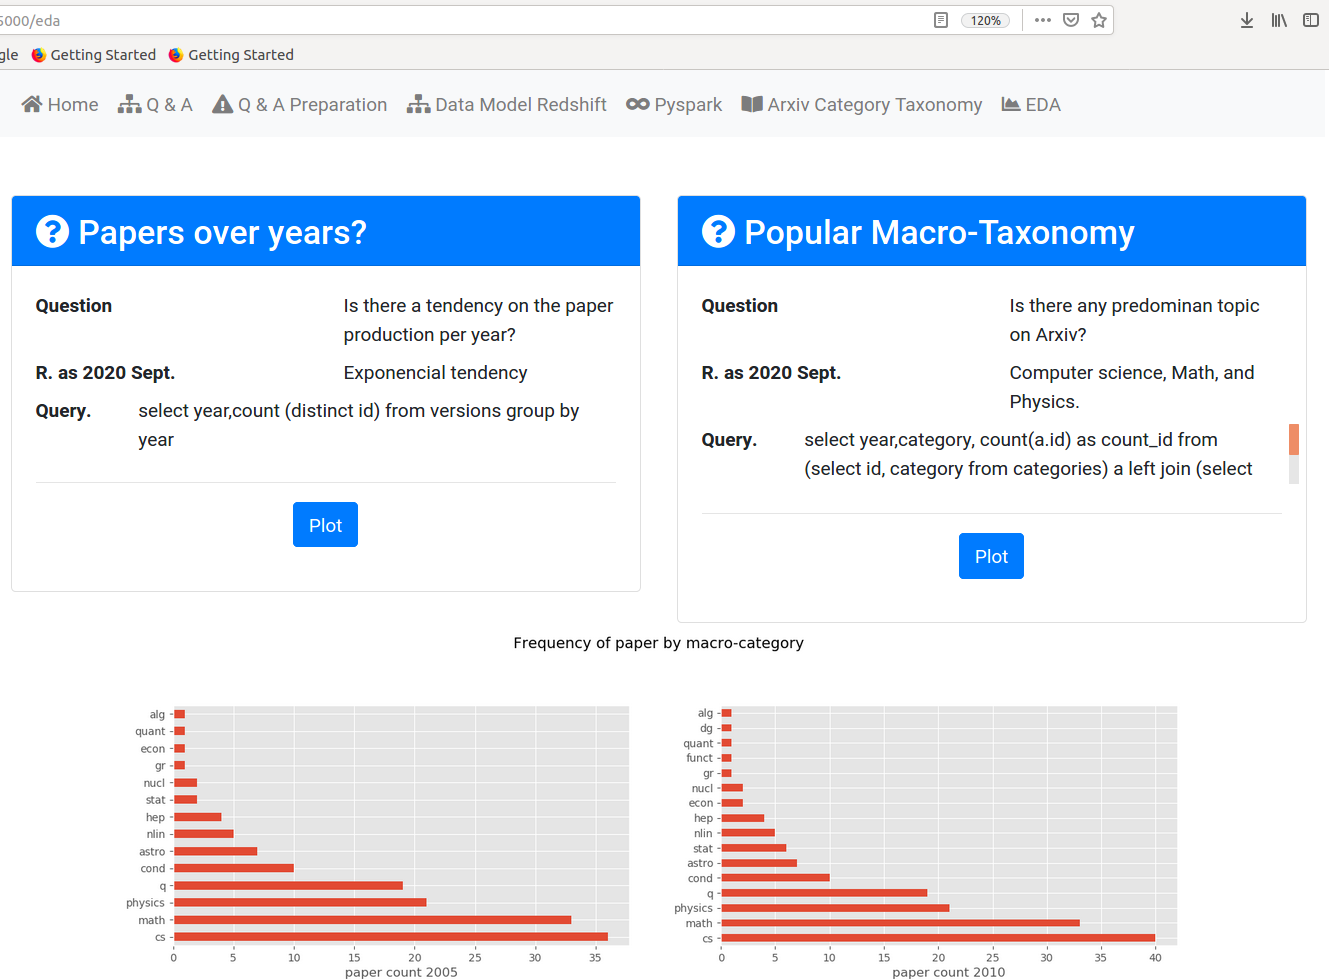
\includegraphics[width=1\linewidth]{images/4_eda}
\caption{Exploratory plots on Database.}
\label{fig:4_eda}
\end{figure}


\begin{figure}
\centering
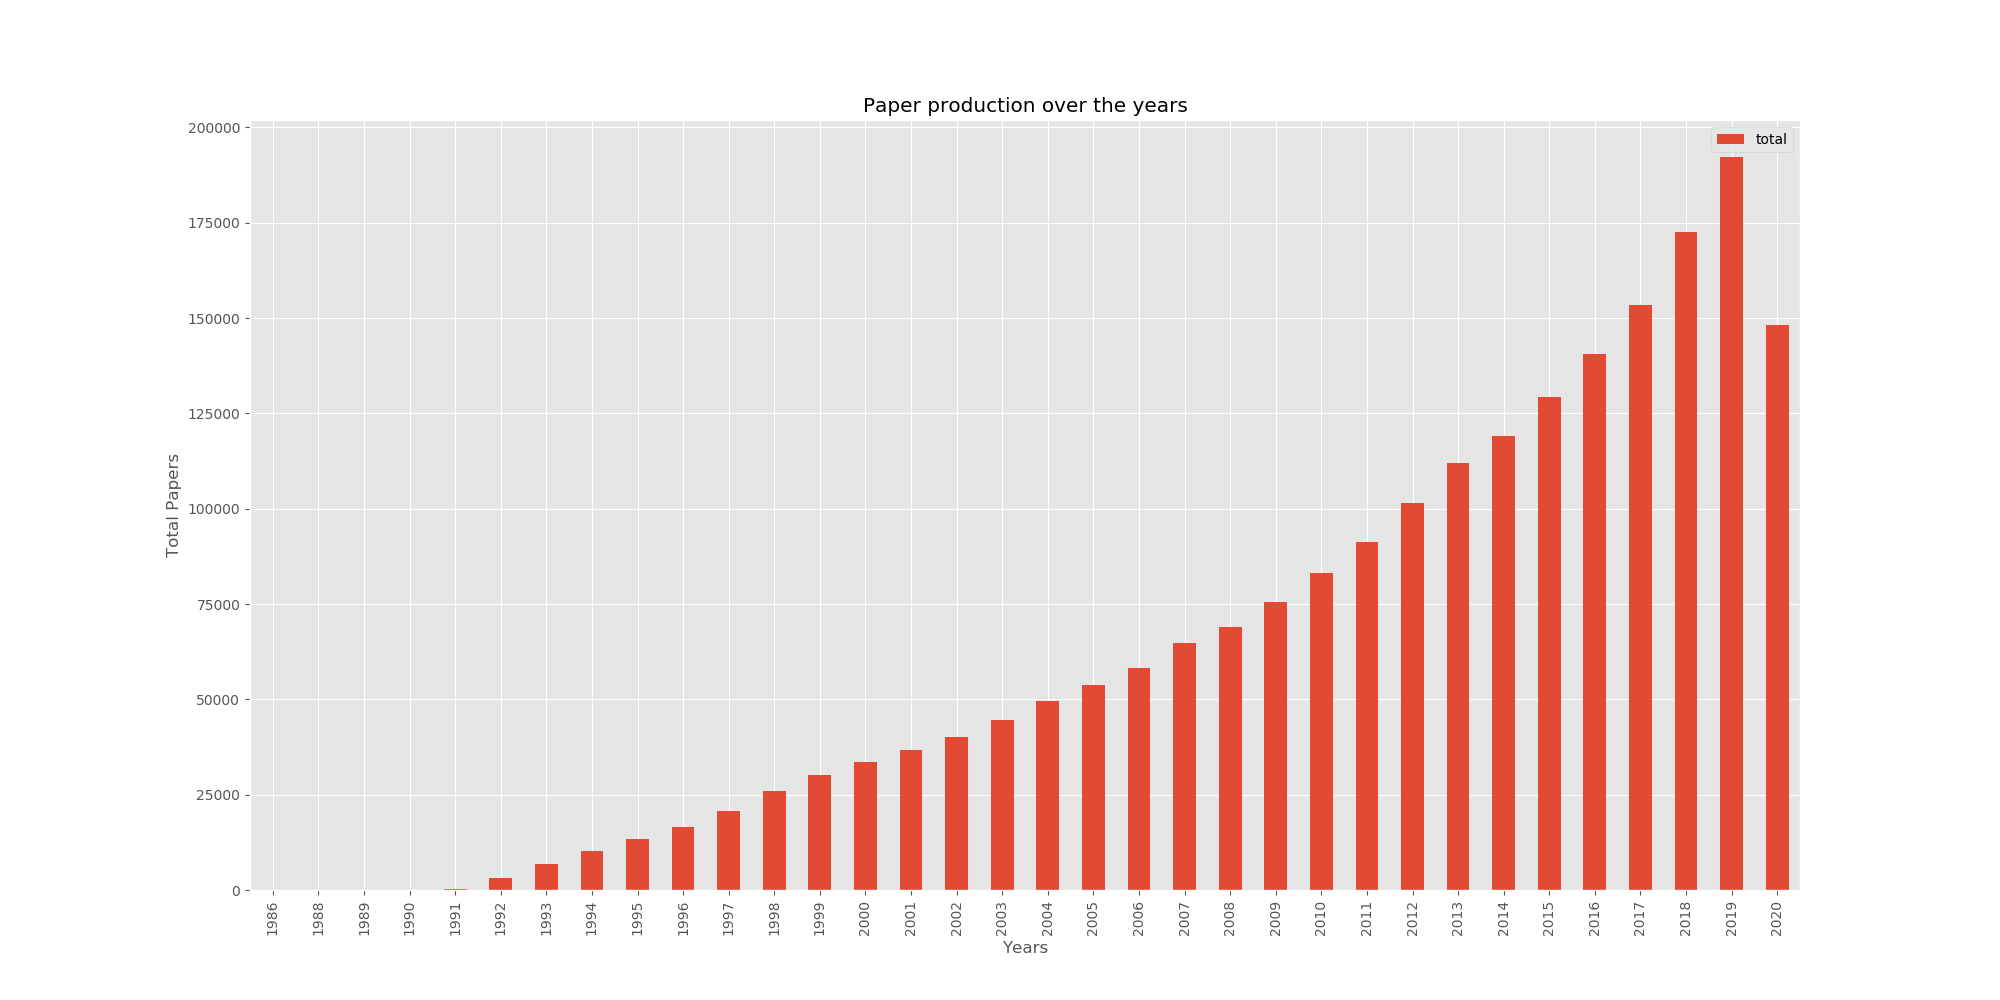
\includegraphics[width=1\linewidth]{images/paper_prod}
\caption{Paper production per year as Sept.2020}
\label{fig:paper_prod}
\end{figure}


\begin{figure}
\centering
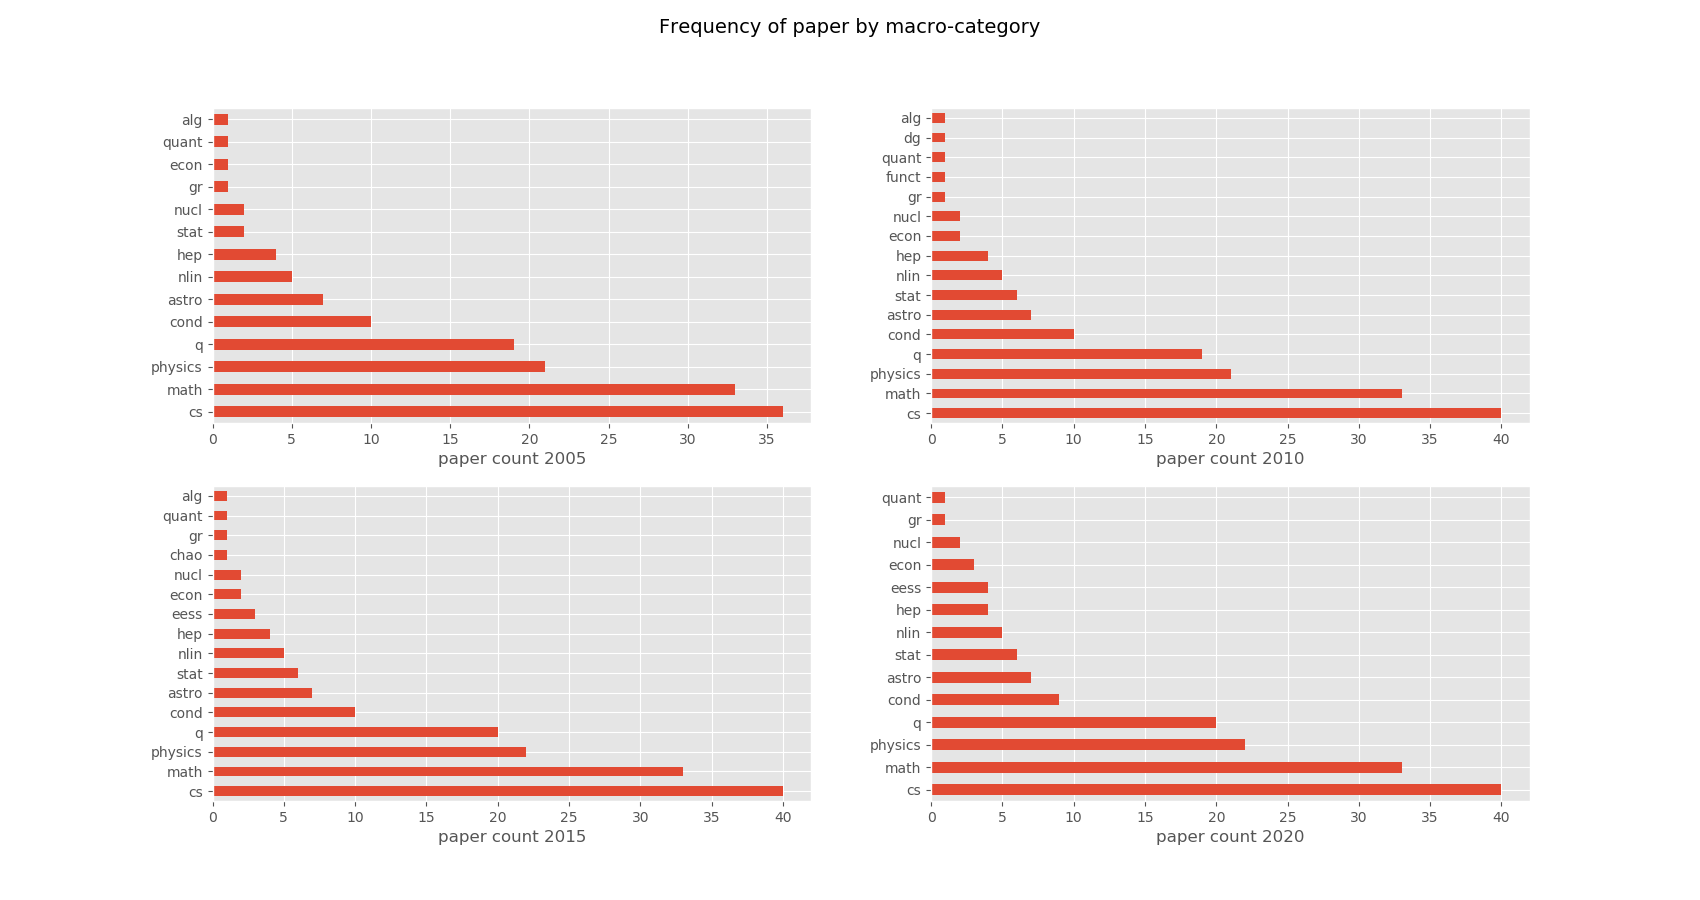
\includegraphics[width=1\linewidth]{images/paper_topics}
\caption{Popular topics in 2000 20010 2015 2020}
\label{fig:paper_topics}
\end{figure}

\subsection{Raw Volume and Uniqueness of the datasets.}

From listing \ref{vol} we can see that in ArXiv dataset there are 3 papers duplicated, whereas NIPS has none. On listing \ref{integrity}
we can observe that there ArXiv contains 32982 rows completed informed, however we more interested on the abstracts of the papers, and the id. 
By constraining the null statement, we now have 1753042 row informed. NIPS has all the row filled. 

\begin{mdframed}[backgroundcolor=light-gray, roundcorner=10pt,leftmargin=1, rightmargin=1, innerleftmargin=15, innertopmargin=15,innerbottommargin=15, outerlinewidth=1, linecolor=light-gray]
\begin{lstlisting}[caption={Volume and Uniqueness},label={vol}]  
>>> df_arxiv = spark.read.json(input_data_1)
>>> df_arxiv.persist()
>>> df_papers_nips = spark.read.format("csv")...
>>> df_arxiv.select("id").distinct().count()
1753039                                                                         
>>> df_arxiv.select("id").count()
1753042                                                                         
>>> df_papers_nips.select("id").distinct().count()
3946
>>> df_papers_nips.select("id").count()
3946
\end{lstlisting}
\end{mdframed} 

\begin{mdframed}[backgroundcolor=light-gray, roundcorner=10pt,leftmargin=1, rightmargin=1, innerleftmargin=15, innertopmargin=15,innerbottommargin=15, outerlinewidth=1, linecolor=light-gray]
\begin{lstlisting}[caption={Completeness of the Datastsets},label={completeness}]  
>>> df_arxiv.dropna().count()
32982                                                                           
>>> df_arxiv.dropna(subset=('id','abstract')).count()
1753042                                                                         
>>> df_papers_nips.dropna().count()
3924
\end{lstlisting}
\end{mdframed} 

\subsection{Assessment}
Since both data sets come from kaggle, they have great quality. Additionally, constraints on redshift enforce primary key uniqueness and nullity, so
no further quality were required.

\section{Application Architecture and Workflow.}











